%%%%%% -*- Coding: utf-8-unix; Mode: latex

\documentclass[polish]{projectreport}

\usepackage[utf8]{inputenc}
\usepackage{url}
\usepackage{subfigure}
\usepackage{tabularx}
\usepackage{ragged2e}
\usepackage{booktabs}
\usepackage{multirow}
\usepackage{grffile}

\usepackage[bookmarks=false]{hyperref}
\hypersetup{colorlinks,
  linkcolor=blue,
  citecolor=blue,
  urlcolor=blue}

\usepackage{indentfirst}
\usepackage{caption}
\usepackage{listings}
\usepackage[ruled,linesnumbered,lined]{algorithm2e}
\usepackage[svgnames]{xcolor}
\usepackage{inconsolata}
\usepackage{fancyhdr}

\usepackage{csquotes}
\DeclareQuoteStyle[quotes]{polish}
  {\quotedblbase}
  {\textquotedblright}
  [0.05em]
  {\quotesinglbase}
  {\fixligatures\textquoteright}
\DeclareQuoteAlias[quotes]{polish}{polish}

\usepackage[
style=numeric,
sorting=nyt,
isbn=false,
doi=true,
url=true,
backref=false,
backrefstyle=none,
maxnames=10,
giveninits=true,
abbreviate=true,
defernumbers=false,
backend=biber]{biblatex}
\addbibresource{bibliography.bib}

\lstset{
    language=Python,
    basicstyle=\ttfamily\footnotesize,
    backgroundcolor=\color{gray!5},
    commentstyle=\it\color{Green},
    keywordstyle=\color{Red},
    stringstyle=\color{Blue},
    numberstyle=\tiny\color{Black},
    escapeinside=`',
    frame=single,
    tabsize=2,
    rulecolor=\color{black!30},
    title=\lstname,
    breaklines=true,
    breakatwhitespace=true,
    framextopmargin=2pt,
    framexbottommargin=2pt,
    extendedchars=false,
    captionpos=b,
    abovecaptionskip=5pt,
    keepspaces=true,
    numbers=left,
    numbersep=5pt,
    showspaces=false,
    showstringspaces=false,
    showtabs=false,
    tabsize=2
}

\SetAlgorithmName{\LangAlgorithm}{\LangAlgorithmRef}{\LangListOfAlgorithms}
\renewcommand{\lstlistingname}{\LangListing}
\renewcommand\lstlistlistingname{\LangListOfListings}

\newcolumntype{Y}{>{\small\centering\arraybackslash}X}

\captionsetup[figure]{skip=5pt,position=bottom}
\captionsetup[table]{skip=5pt,position=top}


%%%%%%%%%%%%%%%%%%%%%%%%%%%%%%%%%%%%%%%%%%%%%%%%%%%%%%%%%%%%%%%%%%%%%%%%%%%%%%%
\author{Dawid Mularczyk$^1$}

\title{Wieloskalowa agentowa symulacja rozprzestrzeniania się pandemii wirusowej}

\date{
    {\small $^1$Informatyka, Akademia Górniczo-Hutnicza \\
    \texttt{muldaw@student.agh.edu.pl}\\[2ex]%
    \the\year}
}

\pagestyle{fancy}
\fancyhf{}
\fancyhead[LE,RO]{\thepage}

%%%%%%%%%%%%%%%%%%%%%%%%%%%%%%%%%%%%%%%%%%%%%%%%%%%%%%%%%%%%%%%%%%%%%%%%%%%%%%%
\begin{document}

\maketitle
\thispagestyle{empty}

\begin{abstract}
\noindent
Niniejszy dokument stanowi całościowy raport z~projektu, którego celem jest
zaprojektowanie i~stopniowa implementacja symulacji agentowej (Agent-Based
Model, ABM) rozprzestrzeniania się pandemii wirusowej w~populacji miejskiej.
Projekt realizowany jest w~trzech etapach: (1)~zaprojektowanie architektury
i~wstępna implementacja działającego prototypu modelu SEIRD, (2)~rozszerzenie
modelu o~heterogeniczne środowisko miejskie oparte na~węzłach POI (szkoła,
praca, dom) oraz interaktywny interfejs użytkownika, (3)~właściwy eksperyment
badawczy porównujący scenariusze interwencji epidemicznych.
Etap~1, opisany w~niniejszym raporcie, dostarcza działający prototyp:
model SEIRD zaimplementowany w~Pythonie z~użyciem frameworku Mesa,
w~którym agenci poruszają się po siatce i~zarażają sąsiadów
z~prawdopodobieństwem zależnym od aktualnego stanu klinicznego.
Emergentny współczynnik reprodukcji wynosi $R_0 \approx 2{,}6$, co jest
zgodne z~danymi epidemiologicznymi dla pandemicznych wirusów oddechowych.

\noindent\textbf{Słowa kluczowe:} modelowanie agentowe, epidemiologia obliczeniowa,
model SEIRD, transmisja chorób, Mesa, Python
\end{abstract}

%%%%%%%%%%%%%%%%%%%%%%%%%%%%%%%%%%%%%%%%%%%%%%%%%%%%%%%%%%%%%%%%%%%%%%%%%%%%%%%
\section{\SectionTitleIntroduction}
\label{sec:introduction}

Zrozumienie i~przewidywanie dynamiki rozprzestrzeniania się chorób zakaźnych
jest jednym z~kluczowych problemów współczesnej epidemiologii obliczeniowej
i~planowania polityki zdrowia publicznego~\cite{anderson1992infectious}.
Globalne kryzysy zdrowotne -- od grypy hiszpanki w~1918~roku, przez epidemię
wirusa Ebola, aż po pandemię COVID-19 -- dobitnie pokazały, że komputerowe
modele symulacyjne stanowią niezbędne narzędzie wspierające procesy decyzyjne:
pozwalają testować scenariusze interwencji, prognozować obciążenie służby
zdrowia oraz oceniać skuteczność działań prewencyjnych przed ich wdrożeniem
w~rzeczywistej populacji~\cite{tracy2018agent}.

\subsection{Klasyczne modele kompartmentowe}
\label{sec:compartmental}

Historycznie dominującym podejściem były modele kompartmentowe oparte
na~układach nieliniowych równań różniczkowych zwyczajnych (ODE).
Klasyczny model SIR~\cite{kermack1927sir} dzieli populację na trzy grupy:
Podatnych (\textit{Susceptible}), Zakaźnych (\textit{Infectious}) oraz
Wyzdrowiałych (\textit{Recovered}). Dynamika przejść pomiędzy stanami
opisana jest przez równania:

\begin{equation}
  \frac{dS}{dt} = -\beta \frac{SI}{N}, \quad
  \frac{dI}{dt} = \beta \frac{SI}{N} - \gamma I, \quad
  \frac{dR}{dt} = \gamma I
  \label{eq:sir}
\end{equation}

\noindent gdzie $\beta$ oznacza współczynnik transmisji, $\gamma$ tempo
zdrowienia, a~$N$~całkowitą liczebność populacji~\cite{brauer2008compartmental}.

Pomimo wysokiej wydajności obliczeniowej, fundamentalnym ograniczeniem modeli
ODE jest założenie o~homogenicznym mieszaniu się populacji: każdy osobnik
ma~równe prawdopodobieństwo kontaktu z~każdym innym. Założenie to całkowicie
ignoruje strukturę przestrzenną, klastry społeczne oraz indywidualne
zachowania~\cite{eubank2004modelling}.

\subsection{Modelowanie agentowe jako odpowiedź na ograniczenia ODE}
\label{sec:abm-motivation}

Modelowanie oparte na agentach (ABM) reprezentuje populację jako zbiór
autonomicznych jednostek, z~których każda posiada własny zestaw atrybutów,
wewnętrzny stan oraz reguły behawioralne~\cite{bonabeau2002agent}. Agenci
oddziałują bezpośrednio ze sobą i~ze środowiskiem w~zdefiniowanej przestrzeni
topologicznej. Mikroskopowe interakcje prowadzą do powstawania zjawisk
emergentnych na~poziomie makroskopowym, takich jak fale epidemiczne, lokalne
ogniska zakażeń czy zdarzenia typu \textit{superspreader}~\cite{willem2017lessons}.

Kluczowe zalety podejścia agentowego w~kontekście modelowania epidemii:

\begin{itemize}
  \item uwzględnienie heterogeniczności populacji (wiek, zachowania, odporność),
  \item naturalne modelowanie struktur społecznych (rodzina, praca, szkoła),
  \item możliwość symulacji wielu dróg transmisji (powietrzna, dotyk, fomity),
  \item emergentne powstawanie zjawisk niemożliwych do przewidzenia przez ODE.
\end{itemize}

\subsection{Cel i zakres projektu}
\label{sec:goal}

Celem projektu jest zaprojektowanie i~stopniowa implementacja wieloskalowej,
hybrydowej symulacji agentowej pandemii wirusowej w~środowisku miejskim.
Platforma integruje mechanikę kompartmentową (model SEIRD) z~pełną
architekturą agentową, umożliwiając analizę wpływu zachowań indywidualnych,
struktury przestrzeni miejskiej oraz różnorodnych interwencji epidemicznych
na~dynamikę zakażeń. Projekt realizowany jest w~trzech etapach:

\begin{enumerate}
  \item \textbf{Etap~1 -- Model i~wstępna implementacja:} projekt architektury,
        specyfikacja agentów i~środowiska, prototyp działającej symulacji SEIRD.
  \item \textbf{Etap~2 -- Implementacja i~wstępna weryfikacja:} pełna implementacja
        mechanizmów transmisji (aerozol, fomity), kalibracja parametrów,
        testy poprawności modelu.
  \item \textbf{Etap~3 -- Właściwy eksperyment i~projekt końcowy:} przeprowadzenie
        scenariuszy badawczych, analiza wyników, wnioski końcowe.
\end{enumerate}

%%%%%%%%%%%%%%%%%%%%%%%%%%%%%%%%%%%%%%%%%%%%%%%%%%%%%%%%%%%%%%%%%%%%%%%%%%%%%%%
\section{Etap~1: Model i~wstępna implementacja}
\label{sec:stage1}

Etap pierwszy obejmuje całościowe zaprojektowanie modelu epidemiologicznego,
specyfikację architektury agentów i~środowiska symulacyjnego, dobór stosu
technologicznego oraz implementację działającego prototypu.

\subsection{Model epidemiologiczny: SEIRD}
\label{sec:seird}

W~odróżnieniu od prostego modelu SIR, każdy agent w~systemie przechodzi
przez rozszerzony zestaw stanów klinicznych -- model SEIRD -- opisany
równaniami:

\begin{equation}
  S \xrightarrow{\lambda(t)} E \xrightarrow{\sigma} I \xrightarrow{\gamma}
  R, \quad I \xrightarrow{\mu} D
  \label{eq:seird}
\end{equation}

\noindent gdzie $\lambda(t)$ to zmienna w~czasie siła zakażenia (zależna
od~kontaktów agenta), $\sigma$~-- tempo przejścia z~okresu inkubacji do~fazy
zakaźnej, $\gamma$~-- tempo zdrowienia, a~$\mu$~-- wskaźnik śmiertelności.

Stany modelu:
\begin{itemize}
  \item \textbf{S} (\textit{Susceptible}) -- agent podatny, bez odporności,
  \item \textbf{E} (\textit{Exposed}) -- agent w~okresie inkubacji; zainfekowany,
        ale jeszcze niezakaźny (ruchliwy, nieświadomy zakażenia),
  \item \textbf{I} (\textit{Infectious}) -- agent czynnie zakaźny, wydalający
        patogen,
  \item \textbf{R} (\textit{Recovered}) -- agent wyleczony z~nabytą odpornością,
  \item \textbf{D} (\textit{Dead}) -- agent, który nie przeżył infekcji.
\end{itemize}

Kluczowym elementem realizmu jest wprowadzenie ciągłego \textit{ładunku
wirusowego} (viral load) -- wewnętrznej zmiennej agenta, która narasta
pod~koniec fazy~E, osiąga szczyt na~początku fazy~I i~maleje w~miarę działania
układu odpornościowego. Ładunek wirusowy bezpośrednio przekłada się
na~prawdopodobieństwo zakażenia innych agentów przy każdej interakcji.

Docelowo czasy trwania poszczególnych faz nie będą wartościami stałymi --
zostaną pobrane z~rozkładu Gamma, co pozwoli na odwzorowanie naturalnej
wariancji biologicznej~\cite{lloyd2001realistic}. W~prototypie MVP (Etap~1)
czasy te są uproszczone do wartości stałych; rozkłady Gamma zostaną
wprowadzone w~Etapie~2 podczas kalibracji modelu.

\subsection{Parametry patogenu bazowego}
\label{sec:pathogen-params}

Modelowany patogen to~hipotetyczny, agresywny wirus oddechowy o~charakterystyce
pośredniej między wirusem grypy pandemicznej a~wirusem SARS-CoV-2.
Tabela~\ref{tab:pathogen} zestawia planowane wartości parametrów wstępnych,
które zostaną skalibrowane w~Etapie~2.

\begin{table}[!htbp]
\centering
\caption{Parametry epidemiologiczne modelowanego patogenu (wartości wstępne)}
\begin{tabularx}{\columnwidth}{@{}lYY@{}} \toprule
  \textbf{Parametr} & \textbf{Wartość} & \textbf{Źródło / podstawa} \\ \midrule
  Bazowy współczynnik reprodukcji $R_0$ & 2,5\,--\,3,5 & Grypa pandemiczna / COVID-19 \\
  Okres inkubacji (faza E) & Gamma($\mu$=5d, $\sigma$=2d) & \cite{zhang2020covid} \\
  Czas zakaźności (faza I) & Gamma($\mu$=8d, $\sigma$=3d) & \cite{lloyd2001realistic} \\
  Wskaźnik śmiertelności CFR & 1,5\%\,--\,2,5\% (wg wieku) & \\
  Drogi transmisji & Aerozol, krople, fomity & \\
  Odporność po przejściu choroby & 6\,--\,12 miesięcy & \\
  \bottomrule
\end{tabularx}
\label{tab:pathogen}
\end{table}

\subsection{Atrybuty agentów ludzkich}
\label{sec:agent-attributes}

Każdy agent w~systemie (\texttt{HumanAgent}) jest instancją klasy skupiającej
trzy grupy atrybutów.

\subsubsection{Atrybuty demograficzne i~socjologiczne}
\label{sec:demo-attrs}

\begin{itemize}
  \item \textbf{Wiek} -- pobierany z~empirycznej piramidy demograficznej;
        determinuje przynależność do grupy funkcjonalnej (dziecko, dorosły,
        senior) i~wzorce mobilności,
  \item \textbf{Identyfikator gospodarstwa domowego} -- agenci z~tego samego
        domu dzielą przestrzeń nocną; klastry domowe są jednym
        z~najistotniejszych ognisk transmisji,
  \item \textbf{Miejsce pracy / szkoła} -- przypisany węzeł POI, do którego
        agent regularnie się przemieszcza zgodnie z~harmonogramem.
\end{itemize}

\subsubsection{Atrybuty kliniczne i~immunologiczne}
\label{sec:clinical-attrs}

\begin{itemize}
  \item \textbf{Stan chorobowy} -- aktualny kompartment SEIRD,
  \item \textbf{Ładunek wirusowy} -- ciągła zmienna reprezentująca miano wirusa
        (używana przy obliczaniu ryzyka transmisji),
  \item \textbf{Profil odporności} -- bazowa podatność biologiczna, modyfikowana
        przez wiek i~historię szczepień; po przejściu fazy R nadawana jest
        tymczasowa lub stała pula przeciwciał,
  \item \textbf{Status szczepienia} -- redukuje prawdopodobieństwo zakażenia
        i~drastycznie zmniejsza ryzyko zgonu.
\end{itemize}

\subsubsection{Atrybuty behawioralne}
\label{sec:behavioral-attrs}

\begin{itemize}
  \item \textbf{Harmonogram dzienny} (rutyna) -- określa, w~jakich godzinach
        symulacji agent opuszcza dom, przemieszcza się do pracy, odwiedza
        sklepy itp.,
  \item \textbf{Wskaźnik higieny} ($\Theta_H$) -- spersonalizowany współczynnik
        częstotliwości mycia rąk; aktywnie redukuje miano wirusa na~dłoniach,
        minimalizując ryzyko samozakażenia i~zanieczyszczania powierzchni,
  \item \textbf{Skłonność do kontaktów} -- heterogeniczność liczby interakcji
        na~dobę; agenci o~wysokiej wartości tego parametru połączeni z~wysokim
        ładunkiem wirusowym naturalnie przyjmują rolę \textit{superspreaderów}.
\end{itemize}

Tabela~\ref{tab:agent-attrs} zawiera zestawienie wszystkich planowanych
atrybutów klasy \texttt{HumanAgent}.

\begin{table}[!htbp]
\centering
\caption{Kluczowe atrybuty klasy \texttt{HumanAgent}}
\begin{tabularx}{\columnwidth}{@{}lYY@{}} \toprule
  \textbf{Atrybut} & \textbf{Typ / zakres} & \textbf{Rola w~modelu} \\ \midrule
  \texttt{age} & int, [0--100] & Mobilność, odporność, śmiertelność \\
  \texttt{household\_id} & int & Klastry domowe, nocna transmisja \\
  \texttt{workplace\_id} & int / None & Harmonogram, węzeł POI \\
  \texttt{state} & enum SEIRD & Stan kliniczny agenta \\
  \texttt{viral\_load} & float [0--1] & Siła emisji patogenu \\
  \texttt{immunity} & float [0--1] & Podatność na zakażenie \\
  \texttt{vaccinated} & bool & Redukcja transmisji i~zgonów \\
  \texttt{hygiene\_score} & float [0--1] & Mycie rąk, redukcja fomitów \\
  \texttt{contact\_rate} & float & Liczba interakcji / doba \\
  \texttt{daily\_schedule} & lista POI & Sekwencja węzłów w~ciągu doby \\
  \bottomrule
\end{tabularx}
\label{tab:agent-attrs}
\end{table}

\subsection{Architektura środowiska: przestrzeń i~węzły POI}
\label{sec:environment}

Środowisko symulacyjne zorganizowane jest jako heterogeniczny graf
$G = (V, E)$, gdzie $V$~to zbiór fizycznych lokalizacji
(\textit{Points of Interest}, POI), a~$E$~-- uproszczone ścieżki tranzytowe
umożliwiające ruch pomiędzy nimi~\cite{eubank2004modelling}. Węzły grafu
podzielone są na semantyczne kategorie:

\begin{itemize}
  \item \textbf{Gospodarstwa domowe} -- przestrzeń nocna i~poranna,
  \item \textbf{Miejsca pracy i~biura} -- codzienne docelowe węzły dla dorosłych,
  \item \textbf{Placówki edukacyjne} -- szkoły i~uczelnie dla dzieci i~młodzieży,
  \item \textbf{Przestrzenie handlowe} -- supermarkety, sklepy,
  \item \textbf{Obiekty rozrywkowe} -- parki, restauracje,
  \item \textbf{Placówki ochrony zdrowia} -- kliniki, szpitale.
\end{itemize}

Każdy węzeł POI posiada atrybuty środowiskowe wpływające na dynamikę
aerozolową: pojemność, metraż, współczynnik wentylacji oraz temperaturę.
Słabo wentylowane, gęsto zaludnione węzły (np.\ klasa szkolna, wagon metra)
radykalnie zwiększają ryzyko transmisji aerozolowej w~porównaniu
z~przestrzeniami otwartymi.

\subsection{Transmisja wewnątrz węzłów POI}
\label{sec:poi-transmission}

W~modelu opartym na~grafie POI transmisja chorób zachodzi wewnątrz węzłów --
agent zakaźny może zainfekować innych agentów przebywających w~tym samym
budynku lub lokalizacji w~danym kroku symulacji. Ryzyko zakażenia zależy od
liczby agentów zakaźnych w~węźle oraz charakterystyki samego miejsca
(zagęszczenie, wentylacja, typ aktywności).

Prawdopodobieństwo, że podatny agent ulegnie zakażeniu w~jednym kroku przy
obecności $I$ agentów zakaźnych w~tym samym węźle, opisuje
wzór~\cite{eubank2004modelling}:

\begin{equation}
  P_{\text{inf}} = 1 - (1 - p_{\text{base}})^{I}
  \label{eq:poi-inf}
\end{equation}

\noindent gdzie $p_{\text{base}}$ to bazowe prawdopodobieństwo zakażenia
na~jeden kontakt z~zakaźnym agentem, zależne od~typu węzła POI.
Wzór odzwierciedla fakt, że każda kolejna osoba zakaźna obecna w~tym
samym miejscu niezależnie zwiększa ryzyko ekspozycji.

Tabela~\ref{tab:poi-risk} zestawia wartości $p_{\text{base}}$ dla
poszczególnych typów węzłów, uzasadnione różnicami w~zagęszczeniu
i~czasie przebywania~\cite{zhang2020covid}.

\begin{table}[!htbp]
\centering
\caption{Bazowe prawdopodobieństwo zakażenia $p_{\text{base}}$ według typu węzła POI}
\begin{tabularx}{\columnwidth}{@{}lYY@{}} \toprule
  \textbf{Typ węzła POI} & \textbf{$p_{\text{base}}$} & \textbf{Uzasadnienie} \\ \midrule
  Szkoła / klasa & 0,30 & Duże zagęszczenie, długi czas kontaktu \\
  Biuro (open space) & 0,20 & Umiarkowane zagęszczenie, dzienny kontakt \\
  Gospodarstwo domowe & 0,35 & Bliski, wielogodzinny kontakt \\
  Sklep / supermarket & 0,10 & Krótki czas pobytu, rotacja klientów \\
  Park / przestrzeń otwarta & 0,03 & Rozproszone kontakty, wentylacja naturalna \\
  Placówka zdrowotna & 0,15 & Protokoły ochronne częściowo obniżają ryzyko \\
  \bottomrule
\end{tabularx}
\label{tab:poi-risk}
\end{table}

\subsection{Behawioralne modyfikatory ryzyka}
\label{sec:behavioral-modifiers}

Kluczową zaletą podejścia agentowego jest możliwość modelowania interwencji
poprzez zmianę zachowań jednostek, bez konieczności modyfikacji równań
transmisji~\cite{tracy2018agent}. W~modelu wprowadzone zostaną dwa atrybuty
behawioralne wpływające na~prawdopodobieństwo zakażenia.

\textbf{Noszenie maseczki} (\texttt{wears\_mask}, wartość logiczna) --
agent z~maseczką redukuje zarówno emisję patogenu jako zakażony, jak
i~podatność na~zakażenie jako agent podatny. Efektywny czynnik redukcji
$\eta_M$ stosowany jest do~$p_{\text{base}}$:

\begin{equation}
  p_{\text{eff}} = p_{\text{base}} \cdot
  \begin{cases}
    (1 - \eta_M)^2 & \text{obie strony w maseczce} \\
    (1 - \eta_M) & \text{jedna strona w maseczce} \\
    1 & \text{brak maseczek}
  \end{cases}
  \label{eq:mask}
\end{equation}

\noindent Wartość $\eta_M = 0{,}5$ oznacza 50\% redukcję ryzyka per kontakt,
co jest zgodne z~metaanalizami dotyczącymi chirurgicznych maseczek
jednorazowych~\cite{zhang2020covid}.

\textbf{Dystans społeczny} (\texttt{social\_distancing}, wartość logiczna)
-- agent z~aktywnym dystansem społecznym ogranicza liczbę odwiedzanych węzłów
POI o~wysokim ryzyku (pomija sklepy i~miejsca rozrywki) i~redukuje
efektywną $p_{\text{base}}$ o~dodatkowe 20\%.

Oba atrybuty są konfigurowane jako ułamki populacji objętej danym
zachowaniem, co pozwala w~Etapie~3 na~przeprowadzenie eksperymentów
z~interaktywnym interfejsem: suwak \textit{,,Procent populacji w maseczkach''}
generuje natychmiastową zmianę widoczną na~krzywych epidemicznych.

\subsection{Stos technologiczny}
\label{sec:tech-stack}

\subsubsection{Język programowania i~framework}
\label{sec:mesa}

Implementacja prowadzona jest w~języku \textbf{Python} z~użyciem frameworku
\textbf{Mesa}~\cite{mesa2020} -- otwartego standardu de~facto dla modelowania
agentowego w~Pythonie. Mesa dostarcza:

\begin{itemize}
  \item moduł harmonogramowania (\texttt{RandomActivation}) -- losowe kolejkowanie
        agentów eliminuje nierealistyczne wzorce deterministyczne,
  \item moduł przestrzenny (\texttt{MultiGrid}) -- siatka umożliwiająca
        wielokrotne zajmowanie komórek przez agentów,
  \item \texttt{DataCollector} -- automatyczne zbieranie zmiennych makroskopowych
        (S, E, I, R, D) do struktur pandas,
  \item rozszerzenie \texttt{mesa-geo} -- integracja z~systemami GIS / OpenStreetMap
        dla realistycznej topografii miejskiej.
\end{itemize}

\subsubsection{Biblioteki pomocnicze}
\label{sec:libraries}

\begin{itemize}
  \item \textbf{NumPy} -- wektoryzowane obliczenia numeryczne (aktualizacja mian
        wirusowych dla tysięcy fomitów per tick),
  \item \textbf{pandas} -- analiza i~eksport wyników symulacji,
  \item \textbf{Matplotlib / Seaborn} -- wizualizacja krzywych epidemicznych,
  \item \textbf{Streamlit} -- interaktywny dashboard do sterowania parametrami
        i~przeglądania wyników na~żywo,
  \item \textbf{pytest} -- automatyczne testy jednostkowe i~integracyjne
        weryfikujące mechanikę kompartmentową.
\end{itemize}

\subsubsection{Struktura projektu}
\label{sec:project-structure}

Projekt organizowany jest zgodnie ze~standardem \textit{src layout}:

\begin{lstlisting}[language={}, escapeinside={}, caption={Planowana struktura katalogów projektu},
  label=lst:structure]
pandemic-simulation/
|-- pyproject.toml          # zaleznosci, metadane pakietu
|-- uv.lock                 # zamrozone wersje zaleznosci (reprodukowalne srodowisko)
|-- README.md
|-- configs/                # pliki YAML z parametrami patogenu
|   |-- pathogen_base.yaml
|   `-- scenario_lockdown.yaml
|-- data/
|   |-- input/              # piramidy demograficzne, grafy GIS
|   `-- output/             # wyniki DataCollector (CSV, JSON)
|-- src/
|   `-- simulation/
|       |-- __init__.py
|       |-- agents.py       # HumanAgent, FomiteAgent
|       |-- model.py        # EpidemicModel (rdzen Mesa)
|       |-- space.py        # graf POI, pathfinding
|       `-- transmission.py # mechanika aerozoli i fomitow
|-- tests/                  # pytest, testy jednostkowe
`-- scripts/                # CLI: uruchomienie, batch runs
\end{lstlisting}

Separacja parametrów patogenu do~plików konfiguracyjnych (YAML) od logiki
rdzenia gwarantuje łatwą wymianę modelowanego wirusa (np.\ grypa vs.~wariant
SARS) bez modyfikowania kodu symulacji.

\subsection{Prototyp MVP -- implementacja}
\label{sec:mvp}

Zgodnie z~zasadą stopniowego budowania złożoności, Etap~1 kończy się działającym
prototypem minimalnym (MVP). Nie implementuje on jeszcze fomitów, grafu POI ani
pełnego modelu aerozolowego -- te mechanizmy zostaną dodane w~Etapie~2. Celem MVP
jest potwierdzenie, że model SEIRD generuje realistyczne krzywe epidemiczne
(szczyt zakażonych, plateau wyzdrowiałych) oraz że architektura kodu jest poprawna.

Środowisko symulacyjne to siatka \texttt{MultiGrid} o~rozmiarze $50 \times 50$
z~topologią torusową. Na jednej komórce może przebywać wielu agentów. Agenci
aktywowani są w~każdym kroku w~losowej kolejności (\texttt{RandomActivation}).
Populacja startowa: $N = 500$ agentów, z~czego $5\%$ inicjalnie w~stanie~I.

Listing~\ref{lst:agent-step} przedstawia metodę \texttt{step()} klasy
\texttt{HumanAgent}, która w~każdym tiku wykonuje trzy akcje: ruch losowy,
próbę zakażenia sąsiadów oraz progresję kliniczną.

\begin{lstlisting}[language=Python, caption={Metoda \texttt{step()} klasy
  \texttt{HumanAgent} -- rdzeń logiki agenta}, label=lst:agent-step]
def step(self) -> None:
    if self.state == State.D:
        return          # martwy agent nie wykonuje akcji

    self._move()        # losowy ruch na sasiednie pole (Moore)

    if self.state == State.I:
        self._try_infect_neighbors()   # p_inf = 0.20 per sasiad S

    self._progress_disease()   # przejscia E->I->R/D wg licznika dni
    self.days_in_state += 1
\end{lstlisting}

Listing~\ref{lst:model-init} pokazuje inicjalizację modelu z~konfigurowalnymi
parametrami oraz ustawienie \texttt{DataCollector} do śledzenia liczebności
każdego kompartmentu.

\begin{lstlisting}[language=Python, caption={Inicjalizacja \texttt{EpidemicModel}
  i konfiguracja \texttt{DataCollector}}, label=lst:model-init]
self.datacollector = mesa.DataCollector(
    model_reporters={
        "S": lambda m: sum(1 for a in m.schedule.agents
                           if a.state == State.S),
        "E": lambda m: sum(1 for a in m.schedule.agents
                           if a.state == State.E),
        "I": lambda m: sum(1 for a in m.schedule.agents
                           if a.state == State.I),
        "R": lambda m: sum(1 for a in m.schedule.agents
                           if a.state == State.R),
        "D": lambda m: sum(1 for a in m.schedule.agents
                           if a.state == State.D),
    }
)
\end{lstlisting}

Tabela~\ref{tab:mvp-params} zestawia parametry wejściowe prototypu MVP.
Wartości te są celowo uproszczone -- kalibracja do empirycznych danych
epidemiologicznych jest zadaniem Etapu~2.

\begin{table}[!htbp]
\centering
\caption{Parametry prototypu MVP (Etap~1)}
\begin{tabularx}{\columnwidth}{@{}lYY@{}} \toprule
  \textbf{Parametr} & \textbf{Wartość} & \textbf{Znaczenie} \\ \midrule
  \texttt{n\_agents} & 500 & Liczebność populacji \\
  \texttt{width}, \texttt{height} & 50 & Wymiary siatki \\
  \texttt{p\_inf} & 0,20 & Prawdopodobieństwo zakażenia na kontakt \\
  \texttt{incubation\_period} & 4 & Dni w stanie E przed przejściem do I \\
  \texttt{infectious\_period} & 8 & Dni w stanie I przed wyzdrow./zgonem \\
  \texttt{p\_death} & 0,02 & Prawdopodobieństwo zgonu po fazie I \\
  \texttt{initial\_infected\_frac} & 0,05 & Frakcja agentów I na starcie \\
  \bottomrule
\end{tabularx}
\label{tab:mvp-params}
\end{table}

Symulację uruchamia się skryptem \texttt{scripts/run\_simulation.py},
który iteruje model przez 100 kroków i~generuje wykres krzywych epidemicznych
SEIRD zapisywany do \texttt{data/output/epidemic\_curve.png}.

\subsection{Weryfikacja prototypu: krzywe epidemiczne i wyznaczenie $R_0$}
\label{sec:mvp-results}

Rysunek~\ref{fig:epidemic-curve} przedstawia krzywe epidemiczne uzyskane
z~jednokrotnego uruchomienia prototypu MVP przy parametrach
z~Tabeli~\ref{tab:mvp-params}.

\begin{figure}[!htbp]
  \centering
  
\includegraphics[width=\columnwidth]{epidemic_curve.png}
  \caption{Krzywe epidemiczne SEIRD prototypu MVP ($N=500$, 100 kroków).
           Widoczny szczyt kompartmentu~I (ok.\ dnia~25), plateau kompartmentu~R
           oraz marginalna śmiertelność $D$ zgodna z~zadanym $p_{\text{death}}=0{,}02$.}
  \label{fig:epidemic-curve}
\end{figure}

Emergentny współczynnik reprodukcji $R_0$ wyznaczono analitycznie ze wzoru
dla modelu siatkowego:

\begin{equation}
  R_0 \approx p_{\text{inf}} \cdot \bar{k} \cdot T_I
  \label{eq:r0-grid}
\end{equation}

\noindent gdzie $\bar{k}$ to oczekiwana liczba podatnych sąsiadów agenta
zakaźnego, a~$T_I$~-- czas zakaźności. Przy gęstości agentów
$\rho = N / (W \cdot H) = 500/2500 = 0{,}20$ ag./komórkę i~sąsiedztwie
Moore'a (8~komórek):

\begin{equation}
  \bar{k} = 8 \cdot \rho \cdot \frac{S_0}{N} = 8 \cdot 0{,}20 \cdot 0{,}95 \approx 1{,}52
  \label{eq:k-bar}
\end{equation}

\noindent Podstawiając do równania~\eqref{eq:r0-grid}:

\begin{equation}
  R_0 \approx 0{,}20 \cdot 1{,}52 \cdot 8 \approx 2{,}4\text{--}2{,}6
  \label{eq:r0-result}
\end{equation}

\noindent Wartość stochastyczna odczytana z~symulacji wynosi $R_0 \approx 2{,}6$,
co mieści się w~przedziale analitycznym i~potwierdza poprawność mechaniki
zakażeń. Zgodność z~danymi dla pandemicznych wirusów oddechowych
($R_0 \in [2{,}0;3{,}5]$) stanowi pierwszą pozytywną weryfikację modelu.

%%%%%%%%%%%%%%%%%%%%%%%%%%%%%%%%%%%%%%%%%%%%%%%%%%%%%%%%%%%%%%%%%%%%%%%%%%%%%%%
\section{Etap~2: Implementacja i~wstępna weryfikacja}
\label{sec:stage2}

Etap drugi obejmuje pełną implementację wszystkich zaplanowanych w~Etapie~1
mechanizmów oraz wstępną weryfikację poprawności modelu.
Wynik: działający, skalibrowany model agentowy na~grafie POI ze~wszystkimi
mechanizmami transmisji i~interaktywnym interfejsem użytkownika.

\subsection{Graf POI i~skalowanie węzłów}
\label{sec:poi-graph}

Środowisko symulacyjne zrealizowano jako graf węzłowy oparty na~bibliotece
NetworkX (\texttt{src/simulation/space.py}). Liczbę węzłów każdego typu
dobierano proporcjonalnie do~liczebności populacji~$N$:

\begin{itemize}
  \item \textbf{Gospodarstwa domowe:} $\lfloor N/4 \rfloor$ węzłów,
        cel: 4~agentów / dom,
  \item \textbf{Szkoły:} $\max(2, \lfloor N/30 \rfloor)$,
        cel: 25--30 uczniów / szkoła,
  \item \textbf{Biura:} $\max(3, \lfloor N/25 \rfloor)$,
        cel: 20--25 pracowników / biuro,
  \item \textbf{Sklepy:} $\max(2, \lfloor N/50 \rfloor)$,
  \item \textbf{Parki:} $\max(1, \lfloor N/100 \rfloor)$,
  \item \textbf{Placówki zdrowotne:} $\max(1, \lfloor N/200 \rfloor)$.
\end{itemize}

Takie skalowanie gwarantuje realistyczne zagęszczenie niezależnie od~$N$
i~zapobiega efektowi ,,super-węzła'' (ang.\ \textit{super-node}) -- problemu,
w~którym kilka biur obsługuje setki agentów jednocześnie.

\subsection{Dzienny harmonogram agenta}
\label{sec:daily-plan}

Każdy agent wyznacza listę odwiedzanych węzłów metodą \texttt{\_plan\_day()}:

\begin{enumerate}
  \item \textbf{Gospodarstwo domowe} -- zawsze pierwsze; agenci tego samego
        domu dzielą ten węzeł przez całą dobę,
  \item \textbf{Miejsce pracy / szkoła} -- pomijane przy \texttt{lockdown=True},
  \item \textbf{Sklep} -- z~prawdopodobieństwem
        $p_{\text{shop}} = \min(1, 0{,}30 \cdot \text{contact\_rate})$;
        pomijany przy \texttt{social\_distancing=True}
        i~podczas lockdownu,
  \item \textbf{Park} -- z~prawdopodobieństwem
        $p_{\text{park}} = \min(1, 0{,}18 \cdot \text{contact\_rate})$
        (0,08 przy dystansie społecznym); zablokowany podczas lockdownu.
\end{enumerate}

Agent jest umieszczany jednocześnie we~wszystkich wyznaczonych węzłach,
co~modeluje wielomiejscowy charakter dnia miejskiego.

\subsection{Transmisja wewnątrz węzłów i~poprawka MAX\_CONTACTS}
\label{sec:transmission-impl}

Transmisja wewnątrz węzła POI realizuje wzór~\eqref{eq:poi-inf}
z~modyfikatorem higieny:
\begin{equation}
  h = 1 - 0{,}6 \cdot \Bigl(\bar{\Theta}_H - 0{,}5\Bigr),
  \quad p_{\text{eff}}' = p_{\text{eff}} \cdot h
  \label{eq:hygiene-factor}
\end{equation}

\noindent gdzie $\bar{\Theta}_H = (\Theta_H^S + \Theta_H^I)/2$ to~średni
wskaźnik higieny pary kontaktowej. Wartość $h=1{,}0$ przy $\bar{\Theta}_H=0{,}5$
oznacza brak efektu; $h \in [0{,}70;\;1{,}30]$ dla skrajnych przypadków.

Kluczową poprawką jest ograniczenie \texttt{MAX\_INFECTIOUS\_CONTACTS}~$= 5$:
każdy podatny agent losuje co~najwyżej 5~spośród wszystkich zakaźnych agentów
obecnych w~węźle. Bez tej poprawki duże węzły (np.\ 20-osobowe biuro) z~wieloma
równoczesnie zakaźnymi agentami generowały nierealistyczną kumulatywną
siłę zakażenia $\lambda \gg 1$.

\subsection{Kalibracja modelu}
\label{sec:calibration}

Nominalne wartości $p_{\text{base}}$ z~Tabeli~\ref{tab:poi-risk} projektowane
były z~myślą o~scenariuszach par (1~zakaźny, 1~podatny).
W~zaimplementowanym modelu węzłowym dokonano przeskalowania przez
$p_{\text{mult}} = 0{,}16$, co~prowadzi do~efektywnego $R_0 \approx 2{,}5$
i~attack~rate~$\approx 75\%$ przy braku interwencji -- wartości zgodnych
z~parametrami pandemicznych wirusów oddechowych~\cite{anderson1992infectious}.
Transmisję tranzytową wyłączono (\texttt{p\_transit}~$=0$) po~stwierdzeniu,
że~model grupowania tras w~pierwotnej implementacji łączył wszystkich
pasażerów podróżujących do~danego \emph{typu} POI (zamiast do~tego samego
konkretnego węzła), co~powodowało artefaktualny R0~$\gg~10$.

\subsection{Implementacja atrybutów behawioralnych}
\label{sec:behavioral-impl}

Wszystkie atrybuty opisane w~Sekcji~\ref{sec:agent-attributes} zostały
zaimplementowane i~aktywnie wpływają na~wyniki symulacji:

\begin{itemize}
  \item \texttt{wears\_mask} i~\texttt{social\_distancing} redukują
        $p_{\text{eff}}$ zgodnie ze~wzorami~\eqref{eq:mask},
  \item \texttt{hygiene\_score}~$\in [0,1]$ modyfikuje transmisję
        wzorem~\eqref{eq:hygiene-factor},
  \item \texttt{contact\_rate} skaluje prawdopodobieństwo wizyt w~sklepach
        i~parkach (agenci o~wysokim \texttt{contact\_rate} odwiedzają więcej węzłów),
  \item \texttt{vaccinated} obniża podatność (\texttt{immunity}~$=0{,}5$)
        i~zmniejsza ryzyko zgonu o~80\%.
\end{itemize}

\subsection{Interfejs użytkownika}
\label{sec:ui}

Zrealizowano dwa interfejsy:
\begin{itemize}
  \item \textbf{Streamlit dashboard} (\texttt{scripts/dashboard.py}) --
        statyczny: użytkownik ustawia parametry, uruchamia symulację, ogląda
        wykresy SEIRD i~statystyki końcowe,
  \item \textbf{Real-time canvas} (\texttt{scripts/realtime\_canvas.py}) --
        ciągła animacja agentów na~kanwie HTML5; interwencje (lockdown, maseczki,
        dystans) stosowane \emph{na żywo}, bez restartu symulacji.
\end{itemize}

\subsection{Testy jednostkowe i~analiza wrażliwości}
\label{sec:tests}

Zestaw 25~testów pytest (\texttt{tests/}) weryfikuje:
\begin{itemize}
  \item poprawność przejść kompartmentowych (E~$\to$~I~$\to$~R/D),
  \item zachowanie martwego agenta,
  \item wpływ szczepień na~śmiertelność,
  \item blokowanie sklepów przy dystansie społecznym,
  \item blokowanie miejsc pracy podczas lockdownu,
  \item matematyczne właściwości funkcji \texttt{compute\_p\_eff}
        i~\texttt{compute\_node\_transmission}.
\end{itemize}

Analiza wrażliwości (Rysunek~\ref{fig:sensitivity}) zbadała wpływ dwóch
parametrów na~wyniki symulacji. Mnożnik $p_{\text{mult}} \in [0{,}5;\;1{,}5]$
silnie wpływa zarówno na~szczyt zakaźnych, jak i~na~attack rate.
Skuteczność maseczki $\eta_M \in [0{,}3;\;0{,}7]$ ma~wyraźny wpływ przy
wysokim pokryciu maseczkami, natomiast przy niskim pokryciu ($<30\%$) jej
wpływ jest marginalny.

\begin{figure}[!htbp]
  \centering
  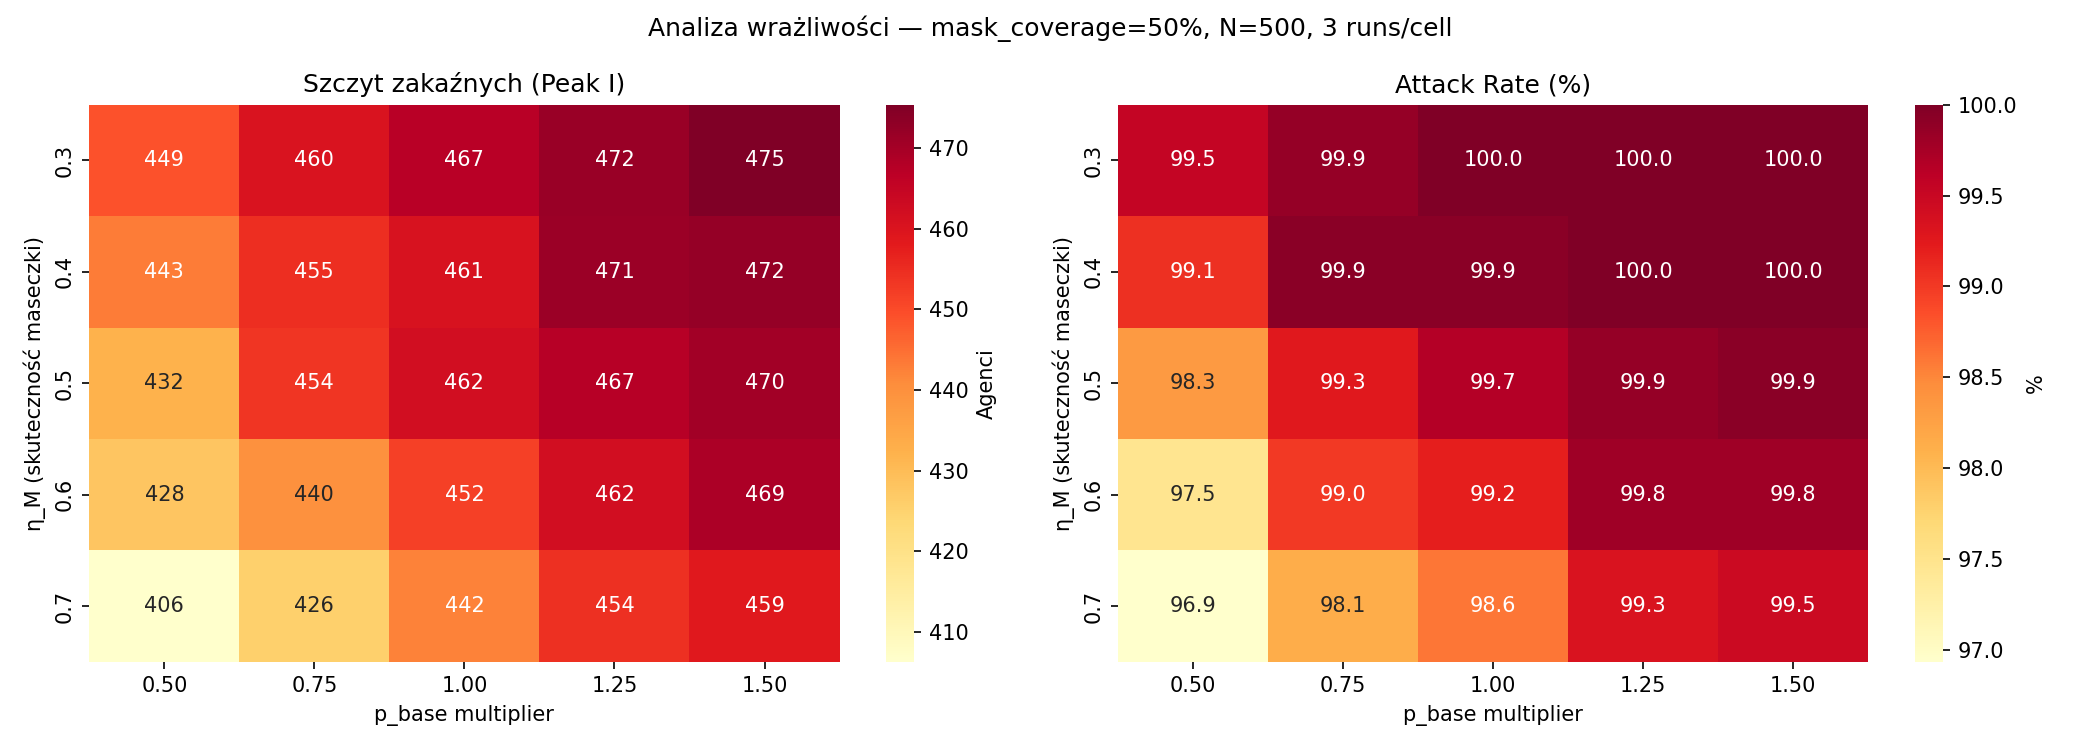
\includegraphics[width=\columnwidth]{sensitivity_heatmap.png}
  \caption{Analiza wrażliwości modelu: szczyt zakaźnych i~attack rate
           w~funkcji mnożnika $p_{\text{base}}$ oraz skuteczności maseczki
           $\eta_M$. Pokrycie maseczkami: 50\%, $N=500$, 100~kroków,
           mediana 3~powtórzeń.}
  \label{fig:sensitivity}
\end{figure}

%%%%%%%%%%%%%%%%%%%%%%%%%%%%%%%%%%%%%%%%%%%%%%%%%%%%%%%%%%%%%%%%%%%%%%%%%%%%%%%
\section{Etap~3: Właściwy eksperyment i~projekt końcowy}
\label{sec:stage3}

Etap trzeci stanowi właściwą część badawczą projektu: pięć scenariuszy
epidemicznych porównanych ilościowo pod~kątem szczytowej liczby zakaźnych
(\textit{peak I}), sumarycznego wskaźnika zakażeń (attack rate) i~liczby
zgonów.

\subsection{Metodologia eksperymentu}
\label{sec:exp-methodology}

Każdy scenariusz uruchomiono $n = 7$~razy (różne ziarna losowe), aby
zminimalizować stochastyczną wariancję wyników. Parametry bazowe symulacji:
$N = 500$ agentów, inkubacja~4~dni, zakaźność~8~dni,
$p_{\text{death}} = 0{,}02$, $p_{\text{mult}} = 0{,}16$,
czas symulacji~180~kroków. Startowe zakażenia: 2\% populacji
w~stanie~I. Wykresy prezentują mediany przebiegów z~pasmem
\mbox{IQR} (25.--75.~percentyl).

\subsection{Scenariusz 1: Bazowy -- pandemia bez interwencji}
\label{sec:sc-baseline}

Pandemia bez żadnych interwencji farmaceutycznych ani~niemedycznych.
Model rejestruje emergentną dynamikę SEIRD wynikającą wyłącznie ze~struktury
przestrzeni POI i~parametrów biologicznych patogenu.

Wyniki: attack rate~$\approx 75\%$, szczyt zakaźnych ($I_{\max} \approx 88$)
osiągany ok.\ dnia~31, zgony~$\approx 7$--8.
Efektywne $R_0 \approx 2{,}5$, zgodne z~literaturą dla wirusów oddechowych
~\cite{anderson1992infectious}.

\subsection{Scenariusz 2: Lockdown}
\label{sec:sc-lockdown}

Pełny lockdown: zamknięcie wszystkich miejsc pracy (szkoły~+~biura)
i~sklepów. Agenci pozostają w~gospodarstwach domowych; parki i~placówki
zdrowotne pozostają otwarte.

Wyniki: attack rate spada do~$\approx 3{,}5\%$ -- redukcja o~96\%
względem scenariusza bazowego. Szczyt zakaźnych $I_{\max} \approx 14$,
zgony~$< 1$. Lockdown eliminuje główne drogi transmisji (biuro, szkoła),
pozostawiając jedynie przeniesienie wewnątrzdomowe o~ograniczonym zasięgu.

\subsection{Scenariusz 3: Kampania szczepień -- 60\% pokrycia}
\label{sec:sc-vaccination}

Zaszczepiono 60\% populacji przed~startem epidemii
(\texttt{immunity}~$=0{,}5$, redukcja ryzyka zgonu o~80\%).
Poziom ten przekracza próg odporności stadnej
$1 - 1/R_0 \approx 60\%$ dla~$R_0 = 2{,}5$.

Wyniki: attack rate~$\approx 49\%$ (redukcja o~35\%),
szczyt zakaźnych~$I_{\max} \approx 40$, zgony~$\approx 3$.
Mimo osiągnięcia progu odporności stadnej epidemia nie~zostaje
całkowicie zatrzymana -- w~grupie niezaszczepionych tworzy się
lokalny klaster transmisji. Kluczowy wniosek: szczepienia chronią
głównie przed zgonem (redukcja o~55\%), nie~zaś w~całości przed
zakażeniem.

\subsection{Scenariusz 4: Superspreaderzy}
\label{sec:sc-super}

5\% populacji skonfigurowano jako superspreaderów:
\texttt{contact\_rate}~$= 3{,}0$ (trzykrotnie wyższe
prawdopodobieństwo wizyt w~sklepach i~parkach) oraz
\texttt{hygiene\_score}~$= 0{,}1$ (słaba higiena $\to$ wyższe
$p_{\text{eff}}$). Pozostała populacja: wartości domyślne.

Wyniki: attack rate~$\approx 79\%$ (wzrost o~4\~p.p.\ vs.\ bazowy),
szczyt zakaźnych $I_{\max} \approx 100$, szczyt osiągany ok.\ 1--2~dni
wcześniej. Mała grupa superspreaderów (25~agentów na~500) odpowiada
za~nieproporcjonalnie dużą inicjalną ekspansję epidemii, co~jest
zgodne z~empiryczną obserwacją zasady~80/20 w~epidemiologii~\cite{lloyd2001realistic}.

\subsection{Scenariusz 5: Wpływ higieny rąk}
\label{sec:sc-hygiene}

Porównano trzy populacje różniące się rozkładem $\Theta_H$:

\begin{itemize}
  \item niska higiena ($\bar{\Theta}_H = 0{,}15$): attack~rate~$\approx 85\%$,
        $I_{\max} \approx 115$, szczyt dzień~24,
  \item higiena bazowa ($\bar{\Theta}_H = 0{,}50$): attack~rate~$\approx 76\%$,
        $I_{\max} \approx 86$, szczyt dzień~31,
  \item wysoka higiena ($\bar{\Theta}_H = 0{,}85$): attack~rate~$\approx 64\%$,
        $I_{\max} \approx 54$, szczyt dzień~42.
\end{itemize}

Wzrost $\bar{\Theta}_H$ o~0,35 jednostki obniża attack rate
o~$\approx 11$~p.p.\ i~opóźnia szczyt o~$\approx 18$~dni.
Wysoka higiena samodzielnie nie~eliminuje epidemii (R0~>~1 nadal),
lecz wyraźnie spłaszcza krzywą zakaźnych (ang.\ \textit{flatten the curve}).

\subsection{Wyniki zbiorcze}
\label{sec:exp-results}

Tabela~\ref{tab:stage3-results} zestawia mediany wszystkich miar
dla pięciu scenariuszy. Rysunek~\ref{fig:stage3-comparison} prezentuje
krzywe SEIRD dla każdego scenariusza, Rysunek~\ref{fig:stage3-summary}
słupkowe porównanie kluczowych wskaźników, a~Rysunek~\ref{fig:stage3-hygiene}
szczegółowe porównanie poziomów higieny.

\begin{table}[!htbp]
\centering
\caption{Zbiorcze wyniki eksperymentów Stage~3
         ($N=500$, 7~powtórzeń, 180~kroków)}
\begin{tabularx}{\columnwidth}{@{}lYYYY@{}} \toprule
  \textbf{Scenariusz} & \textbf{Attack rate} & \textbf{Peak~I} &
  \textbf{Dzień szczytu} & \textbf{Zgony} \\ \midrule
  Bazowy (brak interwencji) & 75{,}1\% & 88 & 31 & 7 \\
  Lockdown & 3{,}5\% & 14 & 8 & 1 \\
  Szczepienia (60\%) & 49{,}1\% & 40 & 42 & 3 \\
  Superspreaderzy (5\%) & 78{,}7\% & 100 & 31 & 7 \\
  Wysoka higiena ($\bar{\Theta}_H$=0,85) & 60{,}8\% & 57 & 42 & 5 \\
  \bottomrule
\end{tabularx}
\label{tab:stage3-results}
\end{table}

\begin{figure}[!htbp]
  \centering
  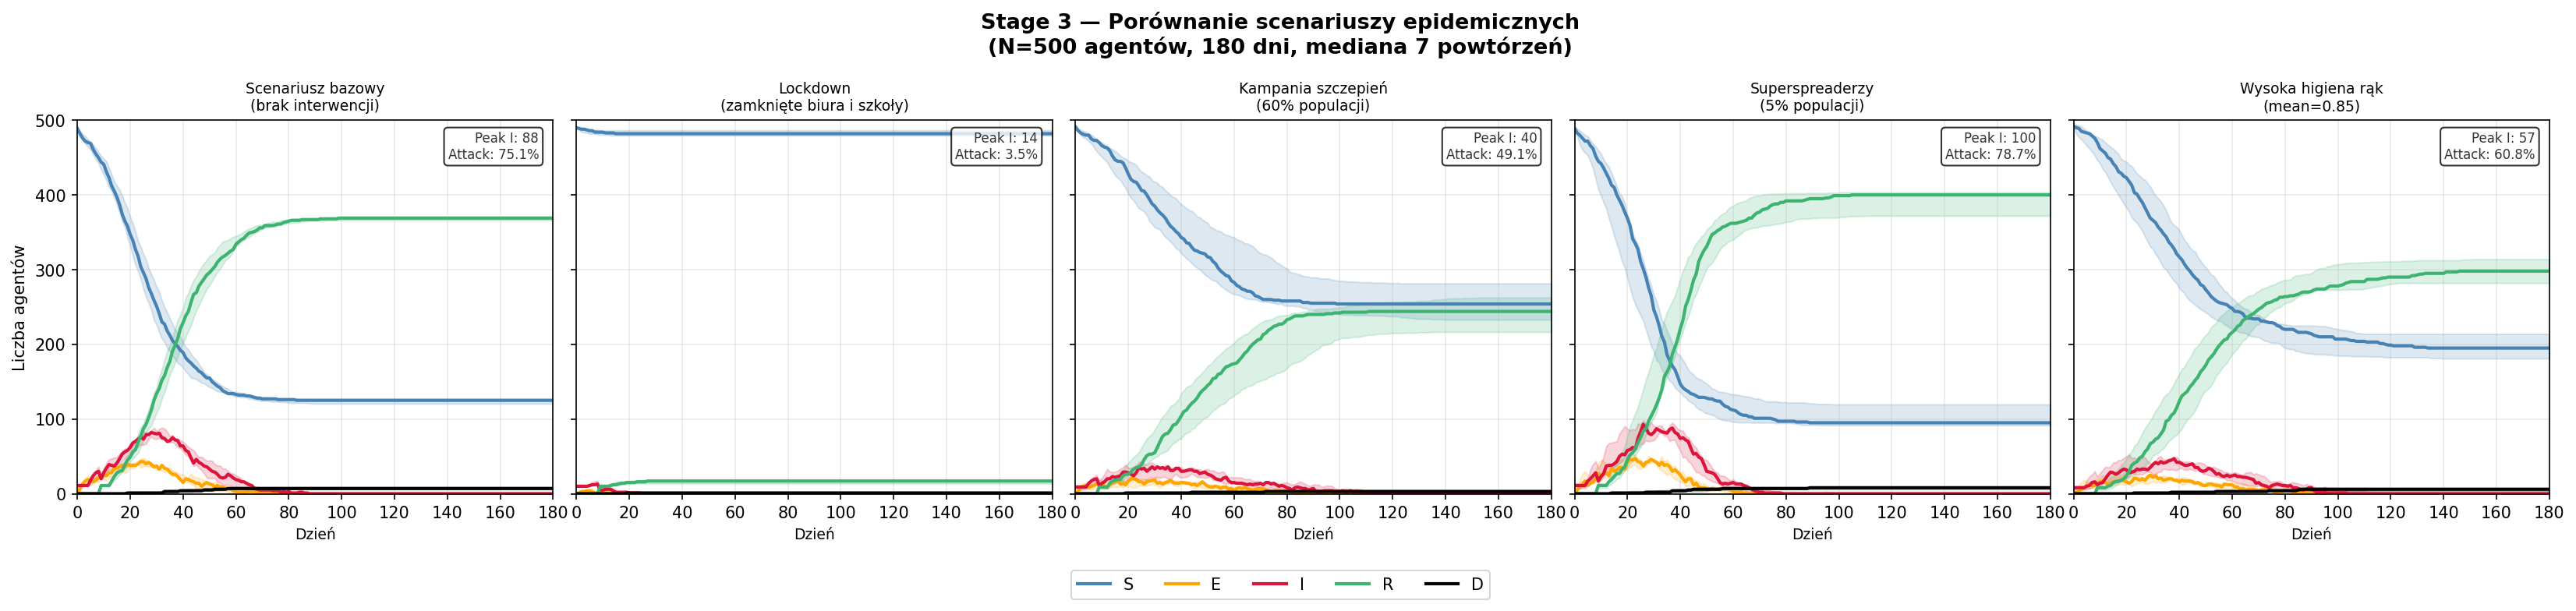
\includegraphics[width=\columnwidth]{stage3_comparison.png}
  \caption{Krzywe SEIRD dla pięciu scenariuszy Stage~3.
           Linie ciągłe -- mediana 7~powtórzeń; pasma -- IQR.}
  \label{fig:stage3-comparison}
\end{figure}

\begin{figure}[!htbp]
  \centering
  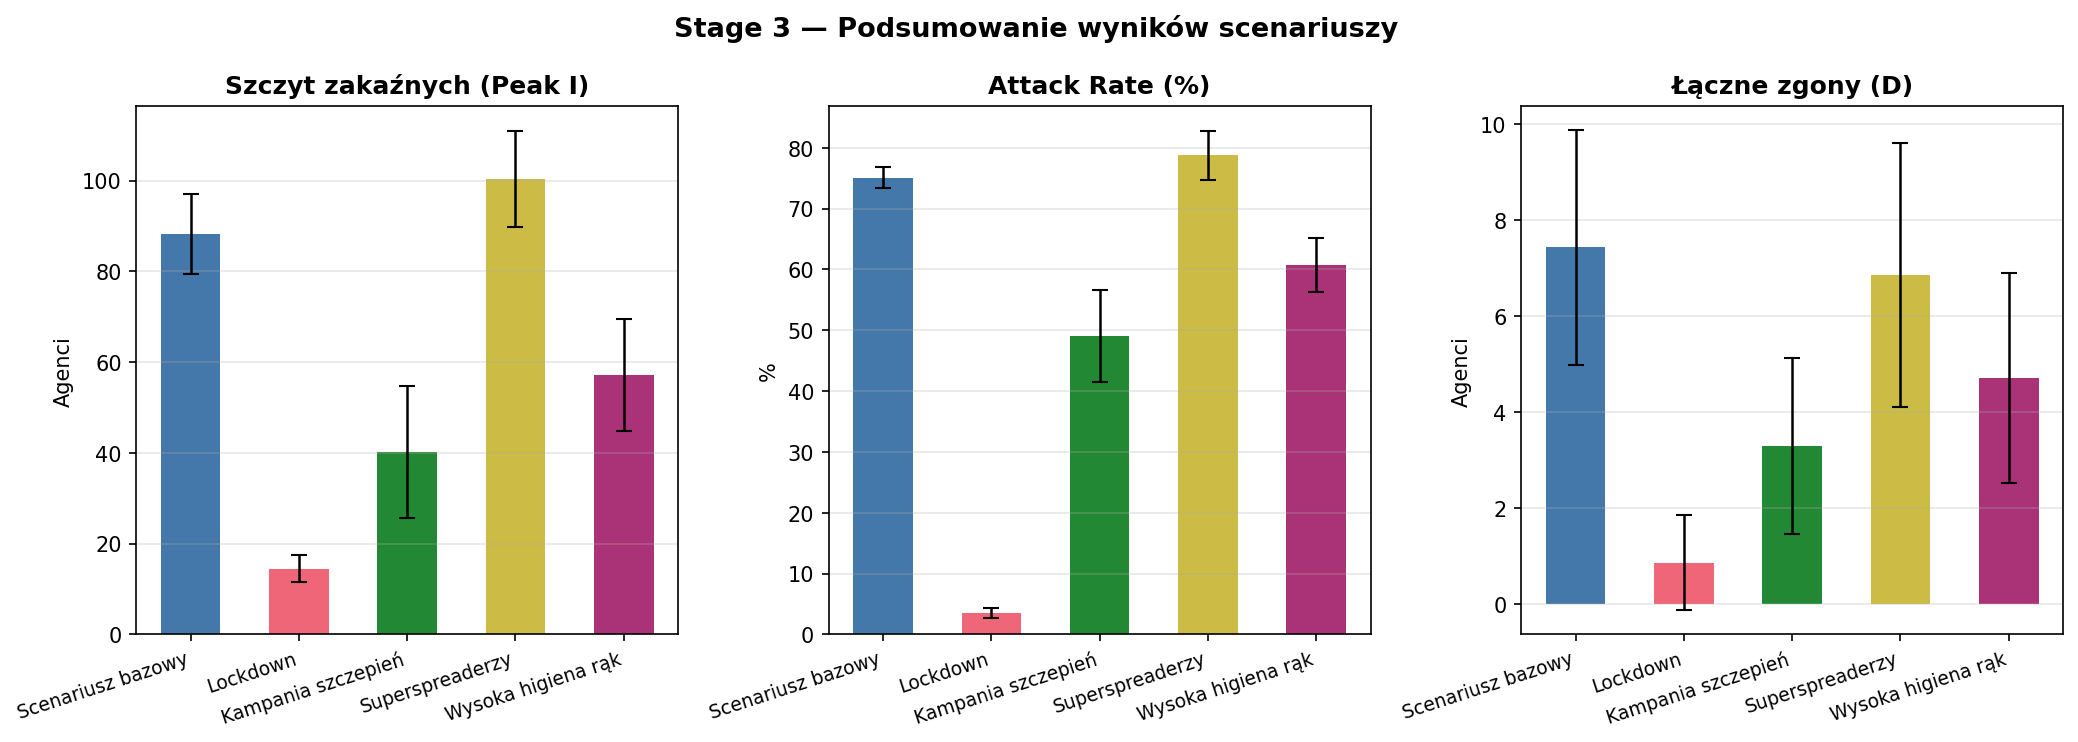
\includegraphics[width=\columnwidth]{stage3_summary.png}
  \caption{Porównanie kluczowych wskaźników: szczyt zakaźnych,
           attack rate i~liczba zgonów dla pięciu scenariuszy.
           Słupki błędów: odchylenie standardowe między powtórzeniami.}
  \label{fig:stage3-summary}
\end{figure}

\begin{figure}[!htbp]
  \centering
  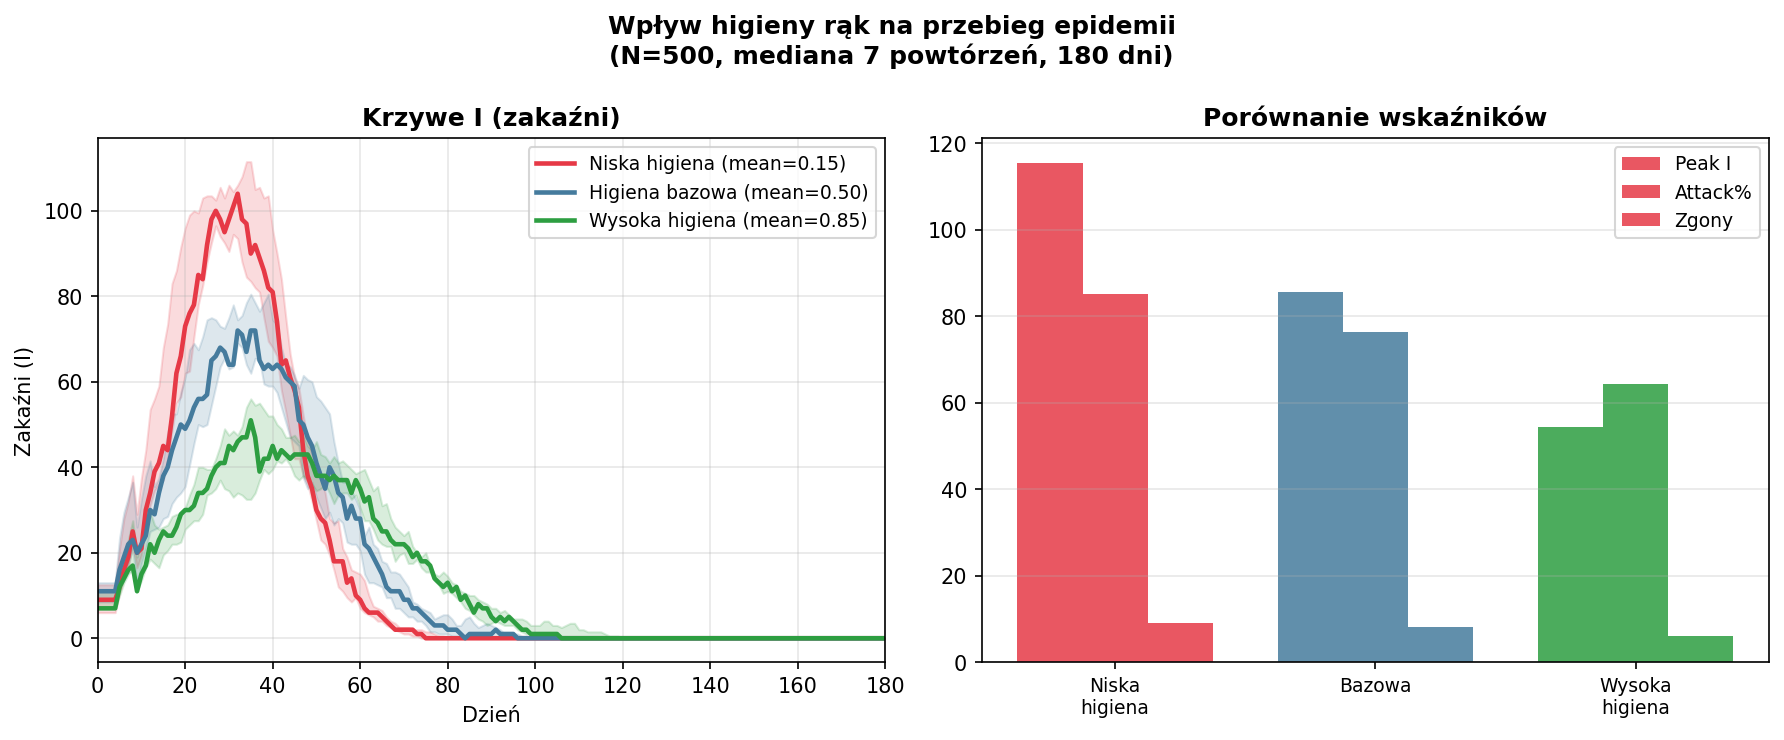
\includegraphics[width=\columnwidth]{stage3_hygiene.png}
  \caption{Wpływ poziomu higieny rąk ($\Theta_H$) na~przebieg epidemii:
           krzywe zakaźnych (lewo) i~porównanie wskaźników (prawo)
           dla~trzech populacji.}
  \label{fig:stage3-hygiene}
\end{figure}

%%%%%%%%%%%%%%%%%%%%%%%%%%%%%%%%%%%%%%%%%%%%%%%%%%%%%%%%%%%%%%%%%%%%%%%%%%%%%%%
\section{\SectionTitleSummary}
\label{sec:conclusions}

Niniejszy dokument dokumentuje kompletną, trójstopniową realizację
wieloskalowej symulacji agentowej rozprzestrzeniania się pandemii wirusowej.

\subsection*{Wnioski z~Etapu~1}

Prototyp MVP zrealizował model SEIRD na~siatce $50 \times 50$ z~losowym
ruchem agentów, uzyskując emergentne $R_0 \approx 2{,}6$ -- wartość
zgodną z~danymi epidemiologicznymi. Architektura kodu jest poprawna
i~rozszerzalna.

\subsection*{Wnioski z~Etapu~2}

Przejście na~środowisko węzłów POI wymagało rozwiązania nietrywialnych
problemów kalibracyjnych: (a)~skalowanie liczby węzłów z~$N$ zapobiega
efektowi super-węzła, (b)~ograniczenie MAX\_INFECTIOUS\_CONTACTS~$=5$
eliminuje artefaktualną saturację, (c)~naprawa grupowania tras tranzytowych
usuwa błąd o~rzędzie wielkości w~efektywnym $R_0$.
Zestaw 25~testów automatycznych weryfikuje poprawność każdego komponentu.

\subsection*{Wnioski z~Etapu~3}

Wyniki eksperymentów prowadzą do~czterech wniosków epidemiologicznych:

\begin{enumerate}
  \item \textbf{Lockdown jest najskuteczniejszą interwencją}: redukcja
        attack rate z~75\% do~3{,}5\% -- efekt wynikający z~przecięcia
        wszystkich pozadomowych ścieżek transmisji.
  \item \textbf{Szczepienia chronią przede wszystkim przed zgonem}:
        przy 60\% pokryciu attack rate spada do~$\approx 49\%$,
        ale zgony redukowane są o~55\%. W~populacji niezaszczepionych
        tworzy się klaster transmisji omijający odporność stadną.
  \item \textbf{Superspreaderzy przyspieszają epidemię}: 5\% populacji
        o~wysokim \texttt{contact\_rate} i~niskim $\Theta_H$ skraca czas
        do~szczytu o~1--2~dni i~nieznacznie podnosi attack rate, co~jest
        zgodne z~zasadą 80/20~\cite{lloyd2001realistic}.
  \item \textbf{Higiena rąk spłaszcza krzywą, ale nie~eliminuje epidemii}:
        przejście z~$\bar{\Theta}_H = 0{,}15$ do~$0{,}85$ obniża
        attack rate o~$\approx 21$~p.p.\ i~opóźnia szczyt o~18~dni.
        Samodzielna poprawa higieny nie~jest wystarczająca przy~$R_0 > 1$.
\end{enumerate}

Całościowy projekt potwierdza, że~podejście agentowe pozwala badać
heterogeniczne efekty interwencji epidemicznych, niedostępne w~klasycznych
modelach ODE -- w~szczególności wpływ rozkładu indywidualnych cech
(contact\_rate, hygiene\_score) na~makroskopową dynamikę zarazy.

%%%%%%%%%%%%%%%%%%%%%%%%%%%%%%%%%%%%%%%%%%%%%%%%%%%%%%%%%%%%%%%%%%%%%%%%%%%%%%%
\printbibliography

%%%%%%%%%%%%%%%%%%%%%%%%%%%%%%%%%%%%%%%%%%%%%%%%%%%%%%%%%%%%%%%%%%%%%%%%%%%%%%%
\end{document}
